% \iffalse meta-comment
%
% Copyright 2016 Brian Dunn
%
% This work may be distributed and/or modified under the
% conditions of the LaTeX Project Public License, either version 1.3
% of this license or (at your option) any later version.
% The latest version of this license is in
%   http://www.latex-project.org/lppl.txt
% and version 1.3 or later is part of all distributions of LaTeX
% version 2005/12/01 or later.
%
% \fi
%
% \iffalse
%<package>\NeedsTeXFormat{LaTeX2e}[1999/12/01]
%<package>\ProvidesPackage{tocdata}
%<package>    [2016/12/02 v0.12 Adds author/artist to TOC entries.]
%
%<*driver>
\documentclass{ltxdoc}


\newcommand{\mypackagename}{tocdata}

\newcommand{\quicksummary}{%
Optionally prints author, artist, or other data on a line
of the \acro{TOC}/\acro{LOF}.
}


\usepackage{lmodern}
% \usepackage{libertine}
\usepackage[T1]{fontenc}
\usepackage[utf8]{inputenc}
\usepackage{textcomp}	% provides \degree, \textquotesingle, \textmu

\usepackage{newunicodechar}
\newunicodechar{ff}{ff}
\newunicodechar{fi}{fi}
\newunicodechar{fl}{fl}
\newunicodechar{ffi}{ffi}
\newunicodechar{ffl}{ffl}
% \newunicodechar{°}{\degree}
\newunicodechar{ρ}{\ensuremath{\rho}}
\newunicodechar{⨯}{\texttimes}
\newunicodechar{⁄}{\textfractionsolidus}
% \newunicodechar{®}{\textregistered}
% \newunicodechar{©}{\textcopyright}
\newunicodechar{—}{---}
\newunicodechar{–}{--}
% \newunicodechar{”}{''}
% \newunicodechar{“}{``}
% \newunicodechar{§}{\S}
% \newunicodechar{¶}{\P}
% \newunicodechar{†}{\dag}
\newunicodechar{‡}{\ddag}

\usepackage{microtype}

\usepackage[log-declarations=false]{xparse}

\usepackage{xifthen}

\usepackage[svgnames]{xcolor}
\definecolor{myurlcolor}{rgb}{0,0,.7}
\definecolor{mylinkcolor}{rgb}{.7,0,0}
\definecolor{codecolor}{rgb}{0,.4,.2}
\definecolor{overviewcolor}{rgb}{0,.2,.4}


\usepackage{graphicx}
\graphicspath{{images/}}

\usepackage{multicol}

\usepackage{enumitem}

\usepackage{array}
\usepackage{longtable}
\usepackage{booktabs}

\usepackage[normalem]{ulem}

% \usepackage{verbatim}
\usepackage{fancyvrb}

\usepackage{comment}
\excludecomment{testing}

% \usepackage{morefloats}
% \usepackage{marginfix}




\usepackage{titletoc}
% \usepackage{tocloft}


\usepackage{titleps}

\newpagestyle{pageheadfoot}{
	\headrule
	\sethead{\pkg{\mypackagename}}{}{\thepage}
% 	\renewcommand{\makefootrule}{\rule[2.5ex]{\linewidth}{.4pt}}
	\setfoot{}{}{}
}

\pagestyle{pageheadfoot}




\usepackage[pdftex,bookmarks=true,hidelinks,%
colorlinks,linkcolor=mylinkcolor,urlcolor=myurlcolor,%
pageanchor=true,hyperindex=false,
]{hyperref}

\hypersetup{%
pdfinfo={%
Title={LaTeX \mypackagename{} package},%
Author={Brian Dunn},%
Subject={LaTeX tocdata package},%
Keywords={LaTeX, tocdata, contents}%
}}


\usepackage{cleveref}



\newcommand{\lmacro}[1]{\textbackslash#1}
\newcommand{\cmds}[1]{\texttt{#1}}
\newcommand{\env}[1]{\texttt{#1}}
\newcommand{\pkg}[1]{\textsf{\textbf{#1}}}
\newcommand{\acro}[1]{\textsc{\lowercase{#1}}}



% Indexing improvements:
\makeatletter

\newcommand*{\Desc@Type}[1]{\raggedleft{\scriptsize#1}\quad}

% \Describe@Usage{name}{margin tag}{index tag}
\newcommand*{\Describe@Usage}[3]{%
% \@bsphack%
\leavevmode\marginpar{\Desc@Type{#2}\texttt{#1}}%
\index{#1\actualchar{\protect\ttfamily#1} (#3)\encapchar usage}%
\index{#3s:\levelchar#1\actualchar{\protect\ttfamily#1}\encapchar usage}%
% \@esphack%
\ignorespaces%
}

% \Describe@CmdUsage{name}{margin tag}{index tag}
% where name is a \macro
\newcommand*{\Describe@CmdUsage}[3]{%
% \@bsphack%
\leavevmode\marginpar{\Desc@Type{#2}\cmd{#1}}%
\SpecialIndex@{#1}{ (#3)\encapchar usage}%
\index{#3s:\levelchar\cmd{#1}\encapchar usage}\ignorespaces%
% \@esphack%
\ignorespaces%
}

\newcommand*{\DescribeCommand}[1]{\Describe@Usage{#1}{Cmd}{command}}
\newcommand*{\DescribeFile}[1]{\Describe@Usage{#1}{File}{file}}
\newcommand*{\DescribePackage}[1]{\Describe@Usage{#1}{Pkg}{package}}
\newcommand*{\DescribeOption}[1]{\Describe@Usage{#1}{Opt}{option}}
\newcommand*{\DescribeArgument}[1]{\Describe@Usage{#1}{Arg}{argument}}
\newcommand*{\DescribeBoolean}[1]{\Describe@Usage{#1}{Bool}{boolean}}
\newcommand*{\DescribeLength}[1]{\Describe@CmdUsage{#1}{Len}{length}}
\newcommand*{\DescribeCounter}[1]{\Describe@Usage{#1}{Ctr}{counter}}
\newcommand*{\DescribeSimple}[1]{\leavevmode\marginpar{\raggedleft\texttt{#1}}\index{#1=\texttt{#1}}\ignorespaces}
\renewcommand{\PrintEnvName}[1]{\strut \MacroFont {\scriptsize{}Env\quad}#1\ }
\renewcommand{\PrintDescribeEnv}[1]{\strut \MacroFont {\scriptsize{}Env\quad}#1\ }

\newcommand*{\DescribeKey}[1]{%
\Describe@Usage{#1}{Key}{key}%
}

\makeatother


\newcommand{\tikz}{Ti\textit{k}z}
\newcommand{\htmlfive}{\acro{HTML}\oldstylenums{5}}
\newcommand{\cssthree}{\acro{CSS}\oldstylenums{3}}

\newcommand{\goesto}{$\Rightarrow$}

\newenvironment{docsidebar}[1][]
{\par\addvspace{1.5ex}%
\hfill\minipage{.9\linewidth}
\raggedright#1
%\smallskip\hrule\medskip
}
{
% \smallskip\hrule
\endminipage\hspace*{\fill}\par\addvspace{1.5ex}}

\makeatletter
\newcommand{\watchout}[1][]{%
\@bsphack%
\marginpar{\hspace*{\fill}
\includegraphics[height=3ex]{symbol_warning.pdf}
\textcolor{DarkRed}{#1}}%
\@esphack%
}
\makeatother




\setlength{\marginparsep}{1em}
\setlength{\marginparpush}{.7ex}
\setlength{\parindent}{0em}
\setlength{\parskip}{2ex}
\setlength{\IndexMin}{40ex}

\usepackage{\mypackagename}

\setcounter{IndexColumns}{2}
\setcounter{GlossaryColumns}{1}

\DisableCrossrefs
\CodelineIndex
\RecordChanges
\begin{document}
  \DocInput{\mypackagename.dtx}
\end{document}
%</driver>
% \fi
%
% \CheckSum{0}
%
% \CharacterTable
% {Upper-case     \A\B\C\D\E\F\G\H\I\J\K\L\M\N\O\P\Q\R\S\T\U\V\W\X\Y\Z
%   Lower-case    \a\b\c\d\e\f\g\h\i\j\k\l\m\n\o\p\q\r\s\t\u\v\w\x\y\z
%   Digits        \0\1\2\3\4\5\6\7\8\9
%   Exclamation   \!     Double quote \"      Hash (number) \#
%   Dollar        \$     Percent       \%     Ampersand     \&
%   Acute accent \'      Left paren    \(     Right paren   \)
%   Asterisk      \*     Plus          \+     Comma         \,
%   Minus         \-     Point         \.     Solidus       \/
%   Colon         \:     Semicolon     \;     Less than     \<
%   Equals        \=     Greater than \>      Question mark \?
%   Commercial at \@     Left bracket \[      Backslash     \\
%   Right bracket \]     Circumflex    \^     Underscore    \_
%   Grave accent \`      Left brace    \{     Vertical bar \|
%   Right brace   \}     Tilde         \~}

% \changes{v0.10}{2016/05/05}{\ 2016/05/05 Initial ver.}
% \changes{v0.11}{2016/07/11}{\ 2016/07/11}
% \changes{v0.11}{2016/07/11}{Minor docs improvements in spelling, grammar, formatting.}
% \changes{v0.12}{2016/12/02}{\ 2016/12/02}



% \GetFileInfo{\mypackagename.sty}
%
% \DoNotIndex{\newcommand,\renewcommand,\addtocounter,\begin,\end,\begingroup,\endgroup}
% \DoNotIndex{\global,\ifbool,\ifthenelse,\isequivalentto,\let}
% \DoNotIndex{\booltrue,\boolfalse}
% \expandafter\DoNotIndex\expandafter{\detokenize{\(,\),\,,\\,\#,\$,\%,\^,\_,\~,\ ,\&,\{,\}}}
%
% ^^A \renewcommand{\listfigurename}{List of }
% \begin{center}
% \thispagestyle{empty}
% \vfill
% ^^A \includegraphics[width=.3\linewidth]{\mypackagename_logo.pdf}
% \vfill
% {\Huge The \textbf{\mypackagename} package}
%
% \fileversion{} --- \filedate
%
% \bigskip
%
% {\small\copyright{} 2016} Brian Dunn\\ \small \texttt{bd@BDTechConcepts.com}
%
% \vspace{.5in}
%
% {\normalsize\textup{\quicksummary}}
%
%
%
% \vfill
%
% \begin{abstract}
% Describes a method for adding information such as an author or artist to
% each line of a table of contents or list of figures entry,
% after the title and just before page number.
% This is commonly done in the table of contents of an anthology, for example.
%
% Support is provided for the \pkg{titletoc} and \pkg{tocloft} packages.
% \end{abstract}
%
% \vspace*{\fill}
% \vspace*{\fill}
% \vspace*{\fill}
% \end{center}
%
% \tableofcontents
% \clearpage
% \listoffigures
% ^^A \listoftables
%
%
% \thispagestyle{pageheadfoot}
%
% \clearpage
%
% \sectionauthor{Introduction}{Brian}{Dunn}
%
% \begin{figure}
% \setlength{\fboxsep}{0pt}
% \centering
% \fbox{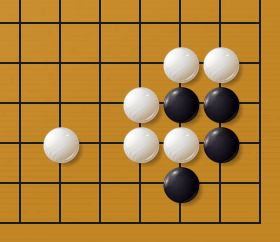
\includegraphics[width=2in]{go_problem.png}}
% \captionartist{The Opening Challenge}
%	[Problem 1-2, from \textit{Gokyo Shumyo}]
%	{Hayashi}{Genbi}
% \end{figure}

%
% Anthologies may be printed with the author alongside each title in the
% table of contents.
%
% Many commonly-recommended methods for doing this with \LaTeX, such as those linked to in
% section \ref{sec:othermethods}, place the author above or below the title and
% page number, but seldom on the same line.
%
% The \pkg{tocdata} package provides some basic infrastructure to help
% add some information to a line in the table of contents, after the title
% and just before the page number.  This function requires the use of either
% the \pkg{titletoc} or \pkg{tocloft} packages.
%
% Additionally,
% user-level macros are provided which add the author's name to a chapter or section,
% and add the artist's name and optional additional text to a figure.
% Author and artist names are also added to the index.
%
% As examples of the use of these high-level macros,
% the major section headings of this documentation
% have the author's name applied, and additional illustrations are supplied as well.
% The results are demonstrated in the table of contents, list of figures, and the index.
%
%
% \clearpage
%
% \sectionauthor[Other methods]{Other methods}{Various}{Authors}
% \label{sec:othermethods}
%
% For other methods which place the author on a separate line from the title, see the
% following.
%
% Note that these methods will be preferable if a larger amount of information
% is to be placed for each title, such that it usually would not all fit on one line
% \watchout[Too much text!]
% in the table of contents.
%
% \href
%	{http://tex.stackexchange.com/questions/47554/add-authors-name-automatically-while-building-toc}
%	{http://tex.stackexchange.com/questions/ \\ \hspace*{1in} 47554/add-authors-name-automatically-while-building-toc}
%
% \href
%	{http://tex.stackexchange.com/questions/110218/add-author-before-chapter-title-in-toc}
%	{http://tex.stackexchange.com/questions/ \\ \hspace*{1in} 110218/add-author-before-chapter-title-in-toc}
%
% \href
%	{http://tex.stackexchange.com/questions/156862/displaying-author-for-each-chapter-in-book}
%	{http://tex.stackexchange.com/questions/ \\ \hspace*{1in} 156862/displaying-author-for-each-chapter-in-book}%
%
% \begin{figure}
% \setlength{\fboxsep}{0pt}
% \centering
% \fbox{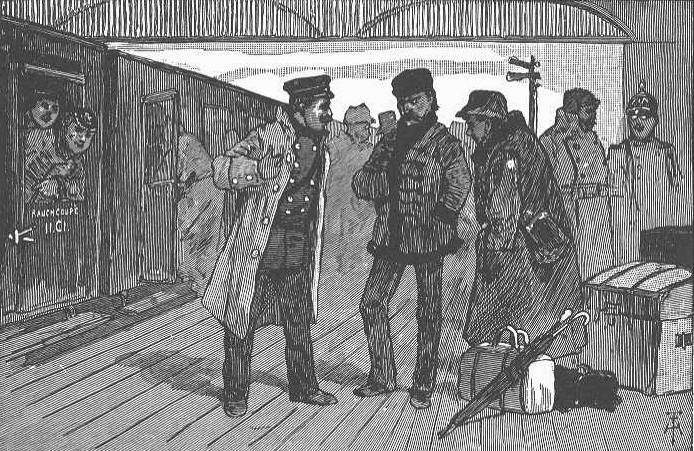
\includegraphics[height=3in]{engineer.jpg}}
% \captionartist
% [The Crazy Engineer]
% {The Crazy Engineer}[Illustration from \textit{The Crazy Engineer} \par \textit{McGuffey's Fifth Eclectic Reader}]{H. F.}{Farny}
% \end{figure}
%
% \clearpage
%
% \begin{figure}
% \centering
% 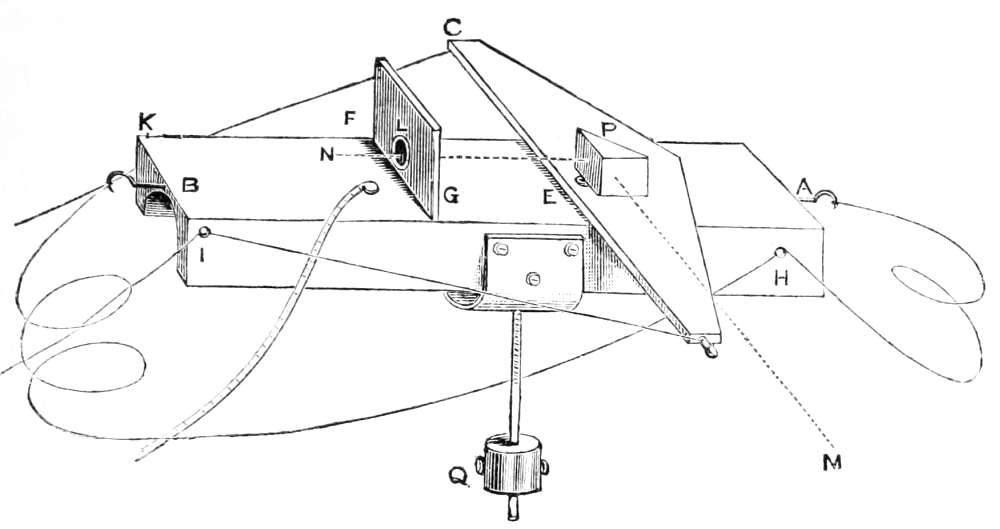
\includegraphics[width=3in]{astronometer_herschel.jpg}
% \captionartist
%	{Astronometer\label{fig:astronometer}}
%	[Astronometer made to compare the light of certain stars by the intervention of the moon.]
%	[Sir]{John}{Herschel}[, 1st Baronet KH FRS]
% \end{figure}
%
% \sectionauthor{How to use \pkg{tocdata}}{Brian}{Dunn}
%
% This section shows how to use the \pkg{tocdata} package.
%
% There are several layers of macros:
% \begin{itemize}
% \item The lowest level provides the basic infrastructure for inserting information
% into the table of contents, along with hooks for the \pkg{titletoc} and \pkg{tocloft} packages.
% \item The intermediate-level macro is \cs{tocdata}, which may be used to manually
% add a piece of data to a \cs{chapter}, \cs{section}, or \cs{caption}.
% \cs{tocdatafont} is also provided to control the appearance of this data in the \acro{TOC}/\acro{LOF}.
% \item At the highest level is a sample implementation of user-level macros which provides
% an easy way to create chapters, sections, and figures with associated authors and artists,
% along with supplemental information for figures, and automatic index entries.
% \end{itemize}
%
%
% \subsection{Basic setup}
%
%
%
% \subsubsection{Preamble}
%
% \pkg{tocdata} requires the use of either the \pkg{tocloft} or \pkg{titletoc} package.
%
% In the preamble, use:
%
%
%	\begin{docsidebar}
%	|\usepackage{tocloft}|
%
%	|\usepackage{tocdata}|
%	\end{docsidebar}
%
%	-\textit{or}-
%
%	\begin{docsidebar}
%	|\usepackage{titletoc}|
%
%	|\usepackage{tocdata}|
%	\end{docsidebar}
%
%
%
%	\begin{docsidebar}
% If using \pkg{titletoc}:
% Note that the user should not use the \cs{dottedcontents} macro, as this
% is not patched for use with \pkg{tocdata}.  Use \cs{titlecontents} instead,
% inserting the \cs{TD@usetocdata} macro as shown below.
%	\end{docsidebar}
% \vspace{-6ex}\watchout[\cs{dottedcontents}]\vspace{6ex}
%
% \subsubsection{Font control in the TOC/LOF}
%
% To control the font used for the author on the table-of-contents line,
% the default is:
%
%	\begin{docsidebar}
%	|\newcommand{\tocdatafont}[1]{{\normalfont\textit{\small#1}}}|
%	\end{docsidebar}
%
%	You may change to other font options, such as:
%
%	\begin{docsidebar}
%	|\renewcommand{\tocdatafont}[1]{\normalfont\textsc{\footnotesize#1}}|
%	\end{docsidebar}
%
%
% \subsection{Mid-level applications}
%
% Should the user only wish to add a bit of text into the \acro{TOC}/\acro{LOF},
% the \cs{tocdata} macro may be used just before the sectioning or caption command,
% as shown next.
%
% \subsubsection{Adding TOC data per section}
% Before each \cs{chapter} or \cs{section} which is to have an author or other data:
%
%	\begin{docsidebar}
%	|\tocdata{toc}{Author's Name}| \\
%	|\chapter{Chapter Title}| \quad -\textit{or}- \quad |\section{Section Title}|
%	\end{docsidebar}
%
%
% \subsubsection{Adding LOF data per figure}
% Before each \cs{caption} which is to have an artist:
%
%	\begin{docsidebar}
%	|\tocdata{lof}{Artist's Name}| \\
%	|\caption{Figure Title}|
%	\end{docsidebar}
%
%	You may wish to print the artist's name in the figure as well.
%
%
% \subsection{High-level user macros}
%
% Additional macros are given in section \ref{sec:usermacros}.
% These are user-level sectioning and captioning commands which add the
% names to the \acro{TOC} and \acro{LOF},
% and also add the artist's name and optional additional text
% to a figure (as in Figure \ref{fig:quail}),
% and also add the names to the index.
% An optional prefix and suffix may be attached to the names (as in Figure \ref{fig:astronometer}),
% and these will be printed at the section heading or caption, but not
% in the \acro{TOC}/\acro{LOF} or in the index.
%
% These macros may be ignored or modified as needed.
%
% \subsubsection{Sectioning commands with authors}
%
% \DescribeMacro{\chapterauthor}
% To use these macros, do not use \cs{tocdata} as shown above, but instead use,
% in the place of \cs{chapter}:
%
% \begin{docsidebar}
% |\chapterauthor[TOC entry]{Title}[Prefix]{First}{Last}[Suffix]|
% \end{docsidebar}
%
% \DescribeMacro{\sectionauthor}
% or, in the place of \cs{section}:
%
% \begin{docsidebar}
% |\sectionauthor[TOC entry]{Title}[Prefix]{First}{Last}[Suffix]|
% \end{docsidebar}
%
% \subsubsection{Figure captions with artist names and add'l text}
%
% \DescribeMacro{\captionartist}
% For figures, in the place of \cs{caption}:
%
% \begin{docsidebar}
% |\captionartist[LOF entry]{Title}[Text][Prefix]{First}{Last}[Suffix]|
% \end{docsidebar}
%
% If you are using the optional prefix, the optional text must also be given, even if it
% is empty.  For example, use:
% \watchout[Optional arguments]
% \begin{docsidebar}
%	|\captionartist{Title}|\textcolor{red}{|[]|}|[Sir]{Isaac}{Newton}|
%
% \medskip
%
% \footnotesize (If only one optional argument is given before the first name, it will be
% interpreted as the optional text, not as the optional prefix.)
% \end{docsidebar}
%
% \DescribeMacro{\captionartist*}
% If you are using the \pkg{caption} package or another package which
% supports \cs{caption*}, you may use \cs{captionartist*} with \pkg{tocdata}.
% The artist and supplemental text will still be printed below the figure,
% and an unnumbered caption will be generated, even though a \acro{LOF} entry will not be made.
%
% Should you mistakenly use \cs{captionartist*} without the \pkg{caption} package,
% expect to get a caption with a visible star in it.
% \watchout[\pkg{caption} package]
% To fix the problem:\\
% \hspace*{1em} |\usepackage{caption}|
%
% \subsubsection{Formatting in sections and figures}
%
% \DescribeMacro{\tocdatachapprint}
% \DescribeMacro{\tocdatasecprint}
% To change the formatting of the author names printed after
% each chapter or section, or to remove them entirely, use
% these macros, as described in section \ref{sec:usermacros} on page \pageref{sec:usermacros}:
%
% 
% \DescribeMacro{\tocdatafigprint}
% \DescribeMacro{\tocdatafigtextprint}
% To change the formatting of a figure's artist's name and optional text,
% use these macros, also described in section \ref{sec:usermacros}.
%
%
% \subsubsection{Text justification}
%
% \DescribeMacro{\tdnamejustify}
% \DescribeMacro{\tdnamecenter}
% \DescribeMacro{\tdnameleft}
% \DescribeMacro{\tdnameright}
% To change the text jusification of the name below a figure, use one of
% the |tdname| macros before the figure.
% All following figures use the selected justification
% until it is changed to another.
%
% \DescribeMacro{\tdtextjustify}
% \DescribeMacro{\tdtextcenter}
% \DescribeMacro{\tdtextleft}
% \DescribeMacro{\tdtextright}
% To change the text jusification of the additional text below a figure, use one of
% the |txtext| macros before the figure.
% All following figures use the selected justification
% until it is changed to another.
%
%
% \StopEventually{\PrintChanges
% \PrintIndex
%
% \begin{figure}[hbp]
% \centering
% \setlength{\fboxsep}{2ex}
% {\fontsize{100}{120}\selectfont$\Omega$}
% \captionartist{Omega --- The End}{Greek}{Alphabet}
% \end{figure}
%}
%
% \begin{figure}[hbp]
% \setlength{\fboxsep}{0pt}
% \centering
% \fbox{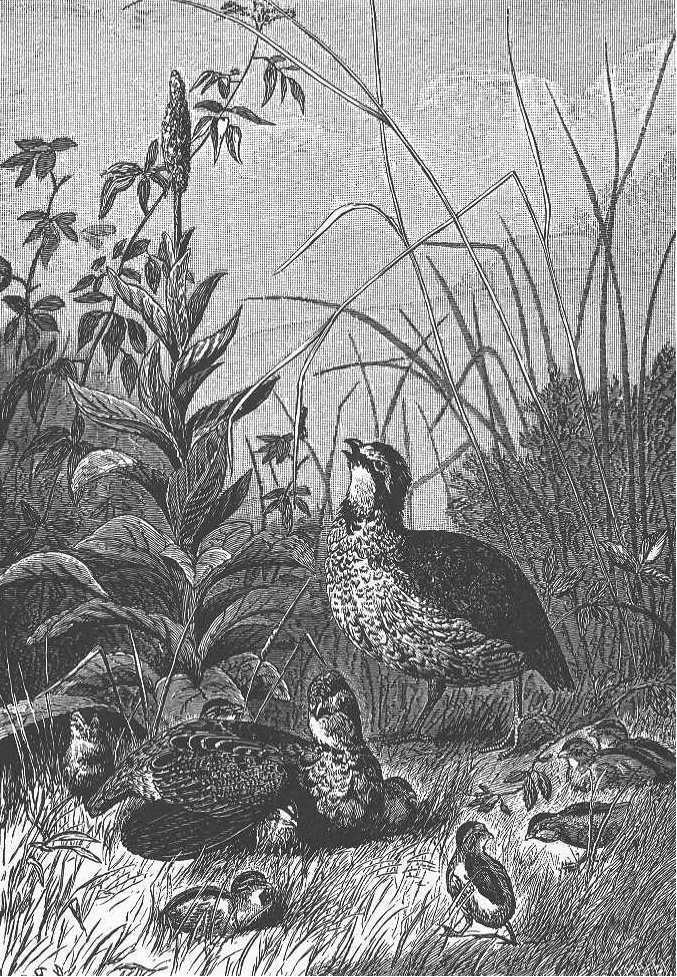
\includegraphics[width=3in]{quail.jpg}}
% \captionartist{Quail\label{fig:quail}}
%	[Illustration from \textit{About Quail} \par \textit{McGuffey's Fifth Eclectic Reader}]
%	{Alexander}{Pope}
% \end{figure}
%
% 
% \clearpage
%
% \sectionauthor{Implementation}{Brian}{Dunn}
%
% \begin{figure}
% \centering
% 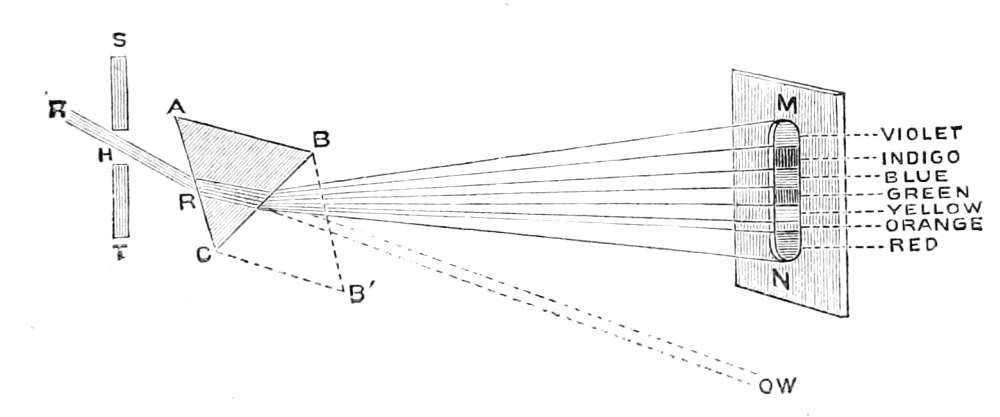
\includegraphics[width=3in]{diagram_sunbeam.jpg}
% \captionartist
%	{Diagram of a Sunbeam}[]
%	[Sir]{Isaac}{Newton}
% \end{figure}
%
% Below, the \pkg{tocdata} code section contains the low-level code used to
% place the data into the table of contents and list of figures, as well as
% the code to control the font used while doing so.
%
% Next are sections used to support \pkg{titletoc} and \pkg{tocloft}.
%
% Finally, the high-level macros are provided.  The user may ignore or redefine these
% as desired.
%
%
% \subsection{Requirements}
%
% \changes{v0.12}{2016/12/02}{Added requirement for \pkg{xifthen}.}
%
%    \begin{macrocode}
\RequirePackage{xparse}
\RequirePackage{etoolbox}
\RequirePackage{xifthen}
%    \end{macrocode}


% \subsection{\pkg{tocdata} code}
% \begin{macro}{\TD@thistocdata}
% Storage for the data to be added to the end of the \acro{TOC} entry:
%    \begin{macrocode}
\newcommand{\TD@thistocdata}{}
%    \end{macrocode}
% \end{macro}

% \begin{macro}{\settocdata}
% Written to the |.toc| or |.lof| file, assigns \cs{thistocdata}:
%    \begin{macrocode}
\newcommand{\settocdata}[1]{\renewcommand{\TD@thistocdata}{#1}}
%    \end{macrocode}
% \end{macro}

% \begin{macro}{\tocdata} \marg{|toc| or |lof|} \marg{text}
%
% To be called by a higher-level macro to assign data to a |.toc| or |.lof| file:
%    \begin{macrocode}
\newcommand{\tocdata}[2]{%
\@bsphack\addtocontents{#1}{\protect\settocdata{#2}}\@esphack%
}
%    \end{macrocode}
% \end{macro}
%
%
% \begin{macro}{\tocdatafont} \marg{text}
%
% Controls the font for the \acro{TOC} data.
%
% |\renewcommand{\tocdatafont}[1]{\textit{#1}}|, etc.
%
%    \begin{macrocode}
\newcommand{\tocdatafont}[1]{{\normalfont\textit{\small#1}}}
%    \end{macrocode}
% \end{macro}
%
%
% \begin{macro}{\TD@usetocdata}
%
% To be inserted into low-level \acro{TOC}-generation code where the data should appear.
%
% See the example using \pkg{titletoc}, below.
%
% Prints the data, then clears the storage so it is not printed again.
%    \begin{macrocode}
\newcommand{\TD@usetocdata}{%
\tocdatafont{\TD@thistocdata}%
\global\def\TD@thistocdata{}%
}
%    \end{macrocode}
% \end{macro}


% \subsection{\pkg{titletoc} support}
%
% \begin{figure}
% \centering
% \setlength{\fboxsep}{2ex}
%
% {\fontsize{140}{160}\selectfont$\pi$}
% \captionartist{Pi --- A Work of Art\label{fig:workofart}}{Greek}{Alphabet}
% \end{figure}
%
%
% If \pkg{titletoc} is loaded, patch macros for its use:
%    \begin{macrocode}
\@ifpackageloaded{titletoc}{
%    \end{macrocode}
%

% \DescribeMacro{\titlecontents}
% A set of \pkg{titletoc} commands which set up the formatting of the
% \acro{TOC} entries.  These are patched to include the tocdata just after
% the leader (|titlerule*|), and just before the page number.
%
% These macros also include spacing commands, and thus may need to be
% redefined by the user.
%
% Note that the user should not use the \cs{dottedcontents} macro, as this
% is not patched for use with \pkg{tocdata}.  Use \cs{titlecontents} instead,
% \watchout[\cs{dottedcontents}]
% inserting the \cs{TD@usetocdata} macro as shown below.
%    \begin{macrocode}
\@ifundefined{chapter}
{}
{
\titlecontents{chapter}[0em]{}{\contentslabel{2.5em}}{}{%
% \dotfill
\titlerule*[.75pc]{.}%
%
%    \end{macrocode}
% The new patch goes here:
%    \begin{macrocode}
\TD@usetocdata% <-- newly added for the tocdata package
%
\contentspage}[\vspace{-.5ex}]%
}
%    \end{macrocode}
% Likewise for sections:
%    \begin{macrocode}
\titlecontents{section}[2.5em]{}{\contentslabel{2.5em}}{}{%
% \dotfill
\titlerule*[.75pc]{.}%
\TD@usetocdata%
\contentspage}[\vspace{-.5ex}]%
%    \end{macrocode}
% Likewise for figures:
%    \begin{macrocode}
\titlecontents{figure}[0em]{}{\contentslabel{3em}}{}{%
% \dotfill
\titlerule*[1pc]{.}%
\TD@usetocdata%
\contentspage}[\vspace{-.5ex}]%
%    \end{macrocode}

%    \begin{macrocode}
}% end of titletoc loaded
{% titletoc is not loaded
}% end of \@ifpackageloaded{titletoc}
%    \end{macrocode}


% \subsection{\pkg{tocloft} support}
%
% If \pkg{tocloft} is loaded, the following patches are applied:
%    \begin{macrocode}
\@ifpackageloaded{tocloft}
{
%    \end{macrocode}
% If the documentclass includes a chapter level:
%    \begin{macrocode}
\if@cfthaschapter
%    \end{macrocode}
% \DescribeMacro{\cftXleader} A set of commands used by \cs{tocloft} to
%	typeset the leader between the title and the page number.
%	These are patched to print the tocdata just after the leader.
%    \begin{macrocode}
\renewcommand{\cftchapleader}{\bfseries\cftdotfill{\cftchapdotsep}\TD@usetocdata}
\renewcommand{\cftsecleader}{\normalfont\cftdotfill{\cftsecdotsep}\TD@usetocdata}
\renewcommand{\cftfigleader}{\normalfont\cftdotfill{\cftfigdotsep}\TD@usetocdata}
\else
%    \end{macrocode}
% If there is no chapter level:
%    \begin{macrocode}
\renewcommand{\cftsecleader}{\bfseries\cftdotfill{\cftsecdotsep}\TD@usetocdata}
\renewcommand{\cftfigleader}{\normalfont\cftdotfill{\cftfigdotsep}\TD@usetocdata}
\fi
}% end of tocloft patches
{}% tocloft not loaded
%    \end{macrocode}

% It is possible to patch the regular \LaTeX{} code here.
% Look at |book.cls| and |article.cls|,
% for the macros \cs{l@chapter} and \cs{l@section}, and look in the \LaTeX{}
% |source2e.pdf| for \cs{\@dottedtocline}.
%
%
%
%
% \clearpage
%
% \subsection{User-level macros}
% \label{sec:usermacros}
%
% \begin{figure}
% \centering
% 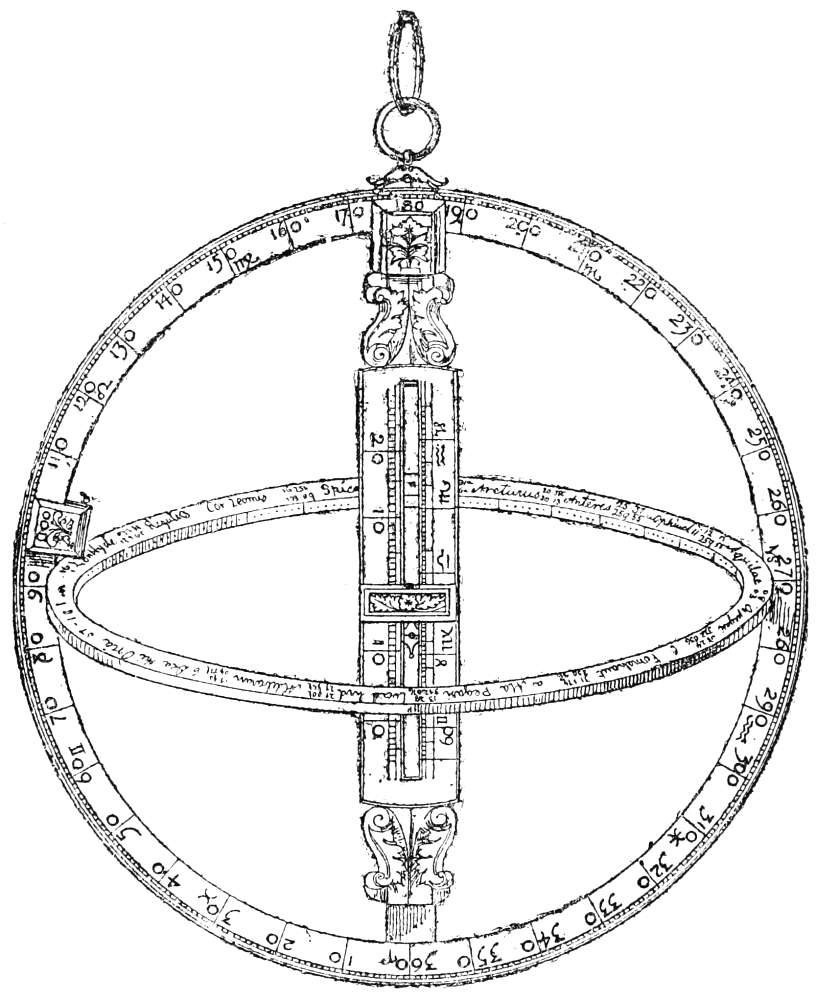
\includegraphics[width=3in]{newton_astrolabe.jpg}
% \captionartist{Sir Isaac Newton's Astrolabe}[][Sir]{Isaac}{Newton}
% \end{figure}
%
%
% Example user-level macros follow.
%
% These macros are in addition to the standard sectioning and caption commands,
% adding first and last names for the table of contents and list of figures.
% For chapters and sections, the author's name with optional prefix and suffix
% are also added below the title.
% For figures, \cs{captionauthor} also prints the figure's artist's
% name with optional prefix and suffix just below the figure.
%
% The regular sectioning and caption commands may still be used for anything
% which does not have an author/artist name.
%
%
% \subsubsection{User customization}
%
%
% \begin{macro}{\TD@optionalname} \marg{name}
%
% Adds optional artist's name and the following space.
%
%    \begin{macrocode}
\newcommand{\TD@optionalname}[1]
{%
\ifthenelse{\equal{#1}{}}%
{}%
{#1~}%
}
%    \end{macrocode}
% \end{macro}
%
%
% \begin{macro}{\tocdatachapprint} \marg{prefix} \marg{first} \marg{last} \marg{suffix}
%
% User-redefinable macro to print the author's name underneath the chapter title.
%
% \changes{v0.12}{2016/11/29}{Improved spacing.}
%
%    \begin{macrocode}
\@ifundefined{chapter}
{}% if no chapters
{% only of chapters exists in this documentclass:
\newcommand{\tocdatachapprint}[4]
{%
\newline\noindent{\normalfont\normalsize\textit{\hspace*{2em}--- %
\TD@optionalname{#1}\TD@optionalname{#2}#3#4}}%
}
}% end of chapters-only
%    \end{macrocode}
% To remove the author's name, redefine this as a null function taking four arguments:
% \begin{docsidebar}
% |\renewcommand{\tocdatachapprint}[4]{}|
% \end{docsidebar}
% \end{macro}
%
% \begin{macro}{\tocdatasecprint} \marg{prefix} \marg{first} \marg{last} \marg{suffix}
%
% User-redefinable macro to print the author's name underneath the section title.
%
% \changes{v0.12}{2016/11/29}{Improved spacing.}
%
%    \begin{macrocode}
\newcommand{\tocdatasecprint}[4]
{%
\newline\noindent{\normalfont\normalsize\textit{\hspace*{2em}--- %
\TD@optionalname{#1}\TD@optionalname{#2}#3#4}%
}%
}
%    \end{macrocode}
% To remove the author's name, redefine this as a null function taking four arguments:
% \begin{docsidebar}
% |\renewcommand{\tocdatasecprint}[4]{}|
% \end{docsidebar}
% \end{macro}
%
%
%
% \begin{macro}{\tocdatafigprint} \marg{prefix} \marg{first} \marg{last} \marg{suffix}
%
% User-redefinable macro to print the artist's name underneath the figure.
%
% \changes{v0.12}{2016/11/29}{Improved spacing.}
% \changes{v0.12}{2016/11/30}{Added name alignment.}
%
%    \begin{macrocode}
\newcommand{\tocdatafigprint}[4]{%
\addvspace{2ex}%
% \addvspace{\medskipamount}%
\begin{minipage}{\linewidth}%
\TD@namealign%
\footnotesize\textsc{{\TD@optionalname{#1}\TD@optionalname{#2}#3#4}}%
\end{minipage}%
\par%
\addvspace{2ex}%
% \addvspace{\medskipamount}%
}
%    \end{macrocode}
% To remove the artist's name, redefine this as a null function taking four arguments:
% \begin{docsidebar}
% |\renewcommand{\tocdatafigprint}[4]{}|
% \end{docsidebar}
% \end{macro}
%
%
%
% \begin{macro}{\tocdatafigtextprint} \marg{first} \marg{last}
%
% User-redefinable macro to print the artist's name underneath the figure.
%
% \changes{v0.12}{2016/11/29}{Improved spacing.}
% \changes{v0.12}{2016/11/29}{Added text alignment.}
%
%    \begin{macrocode}
\newcommand{\tocdatafigtextprint}[1]{%
\addvspace{2ex}%
\begin{minipage}{\linewidth}%
\TD@textalign%
\footnotesize%
\setlength{\parskip}{1.5ex}%
\setlength{\parindent}{0em}%
#1%
\end{minipage}%
\par%
\addvspace{2ex}%
% \addvspace{\medskipamount}%
}
%    \end{macrocode}
% \end{macro}
%
%
%
% \subsubsection{Chapters and sections}
%
% \begin{macro}{\chapterauthor} * \oarg{2:TOC entry} \marg{3:title}
%	\oarg{4:prefix} \marg{5:first} \marg{6:last} \oarg{7:suffix}
%
% \changes{v0.12}{2016/11/28}{Expands first name before index check.}
%    \begin{macrocode}
\@ifundefined{chapter}
{}% if no chapters
{% only of chapters exists in this documentclass:
\NewDocumentCommand{\chapterauthor}{s o m O{} m m O{}}{%
%    \end{macrocode}
% The starred version does not create a \acro{TOC} entry,
% so it is used as-is:
%    \begin{macrocode}
\IfBooleanTF{#1}% star:
{\chapter*{#3\tocdatachapprint{#4}{#5}{#6}{#7}}}%
%    \end{macrocode}
% The un-starred version appears in the \acro{TOC}, so add the author's name:
%    \begin{macrocode}
{% no star:
\tocdata{toc}{#5 #6}%
%    \end{macrocode}
% Create the chapter depending on the optional name:
%    \begin{macrocode}
\IfValueTF{#2}%
{\chapter[#2]{#3\tocdatachapprint{#4}{#5}{#6}{#7}}}%
{\chapter[#3]{#3\tocdatachapprint{#4}{#5}{#6}{#7}}}%
}%
%    \end{macrocode}
% Create an index entry depending on whether there is a first name:
%    \begin{macrocode}
\ifthenelse{\equal{#5}{}}%
{\index{#6}}%
{\index{#6, #5}}%
}% end of \chapterauthor
}% end of \@ifundefined{chapter}
%    \end{macrocode}
% \end{macro}


% \begin{macro}{\sectionauthor} * \oarg{2:TOC entry} \marg{3:title}
%	\oarg{4:prefix} \marg{5:first} \marg{6:last} \oarg{7:suffix}
%
% \changes{v0.12}{2016/11/28}{Expands first name before index check.}
%    \begin{macrocode}
\NewDocumentCommand{\sectionauthor}{s o m O{} m m O{}}{%
%    \end{macrocode}
% The starred version does not create a \acro{TOC} entry,
% so it is simply used as-is:
%    \begin{macrocode}
\IfBooleanTF{#1}% star:
{\section*{#3\tocdatasecprint{#4}{#5}{#6}{#7}}}%
%    \end{macrocode}
% The un-starred version appears in the \acro{TOC}, so add the author's name:
%    \begin{macrocode}
{% no star:
\tocdata{toc}{#5 #6}%
%    \end{macrocode}
% Create the section depending on the optional name:
%    \begin{macrocode}
\IfValueTF{#2}%
{\section[#2]{#3\tocdatasecprint{#4}{#5}{#6}{#7}}}%
{\section[#3]{#3\tocdatasecprint{#4}{#5}{#6}{#7}}}%
}% no star
%    \end{macrocode}
% Create an index entry depending on whether there is a first name:
%    \begin{macrocode}
\ifthenelse{\equal{#5}{}}%
{\index{#6}}%
{\index{#6, #5}}%
}
%    \end{macrocode}
% \end{macro}
%
%
%
% \subsubsection{Figure name alignment}
%
% \begin{macro}{\TD@namealign} Sets text alignment in the optional text.
%    \begin{macrocode}
\newcommand{\TD@namealign}{\centering}
%    \end{macrocode}
% \end{macro}
%
% \begin{macro}{\tdnamejustify} Sets justified text alignment in the optional text.
% \changes{v0.12}{2016/11/30}{etc. Added name alignment.}
%    \begin{macrocode}
\newcommand{\tdnamejustify}{%
\renewcommand{\TD@namealign}{}%
}
%    \end{macrocode}
% \end{macro}
%
% \begin{macro}{tdnamecenter} Sets centered text alignment in the optional text.
%    \begin{macrocode}
\newcommand{\tdnamecenter}{%
\renewcommand{\TD@namealign}{\centering}%
}
%    \end{macrocode}
% \end{macro}
%
% \begin{macro}{tdnameleft} Sets left text alignment in the optional text.
%    \begin{macrocode}
\newcommand{\tdnameleft}{%
\renewcommand{\TD@namealign}{\raggedright}%
}
%    \end{macrocode}
% \end{macro}
%
% \begin{macro}{tdnameright} Sets right text alignment in the optional text.
%    \begin{macrocode}
\newcommand{\tdnameright}{%
\renewcommand{\TD@namealign}{\raggedleft}%
}
%    \end{macrocode}
% \end{macro}
%
%
% \subsubsection{Figure text alignment}
%
% \begin{macro}{\TD@textalign} Sets text alignment in the optional text.
%    \begin{macrocode}
\newcommand{\TD@textalign}{\centering}
%    \end{macrocode}
% \end{macro}
%
% \begin{macro}{\tdtextjustify} Sets justified text alignment in the optional text.
% \changes{v0.12}{2016/11/30}{etc. Added text alignment.}
%    \begin{macrocode}
\newcommand{\tdtextjustify}{%
\renewcommand{\TD@textalign}{}%
}
%    \end{macrocode}
% \end{macro}
%
% \begin{macro}{tdtextcenter} Sets centered text alignment in the optional text.
%    \begin{macrocode}
\newcommand{\tdtextcenter}{%
\renewcommand{\TD@textalign}{\centering}%
}
%    \end{macrocode}
% \end{macro}
%
% \begin{macro}{tdtextleft} Sets left text alignment in the optional text.
%    \begin{macrocode}
\newcommand{\tdtextleft}{%
\renewcommand{\TD@textalign}{\raggedright}%
}
%    \end{macrocode}
% \end{macro}
%
% \begin{macro}{tdtextright} Sets right text alignment in the optional text.
%    \begin{macrocode}
\newcommand{\tdtextright}{%
\renewcommand{\TD@textalign}{\raggedleft}%
}
%    \end{macrocode}
% \end{macro}
%
%
%
% \subsubsection{Figures}
%
% \begin{macro}{\captionartist} * \oarg{2:LOF entry} \marg{3:title}
%	\oarg{4:supplemental text}
%	\oarg{5: prefix} \marg{6:first} \marg{7:last} \oarg{8:suffix}
%
% \changes{v0.12}{2016/11/28}{Allows paragraphs in add'l text.}
% \changes{v0.12}{2016/11/28}{Expands first name before index check.}
%
% This macro adds optional supplemental text, which will be printed below the
% artist's name and above the caption, presuming that the caption is generated
% below the figure.
%
% If using the optional prefix, the optional text must also be given, even if it
% \watchout[Optional arguments]
% is empty.  For example, use:
% \begin{docsidebar}
%	|\captionartist{Title}|\textcolor{red}{|[]|}|[Sir]{Isaac}{Newton}|
%
% \medskip
%
% \footnotesize (If only one optional argument is given before the first name, it will be
% interpreted as the optional text, not as the optional prefix.)
% \end{docsidebar}
%    \begin{macrocode}
\NewDocumentCommand{\captionartist}{s o m +O{} O{} m m O{}}{%
%    \end{macrocode}
% Print the artist's name next to the figure:
%    \begin{macrocode}
\par\addvspace{\medskipamount}%
\tocdatafigprint{#5}{#6}{#7}{#8}%
%    \end{macrocode}
% If supplemental text is provided, print it below the author:
%    \begin{macrocode}
\ifthenelse{\equal{#4}{}}{}{\par\tocdatafigtextprint{#4}}%
%    \end{macrocode}
% Remove any existing vertical space and only use \cs{caption}'s built-in spacing:
%    \begin{macrocode}
\unskip%
%    \end{macrocode}
% If starred, there should be no \acro{TOC} entry, so do not add tocdata.
% Use \cs{caption*} from the \pkg{caption} or similar packages.
%    \begin{macrocode}
\IfBooleanTF{#1}%
{% starred
\IfValueTF{#2}{\caption*[#2]{#3}}{\caption*{#3}}%
}% starred
{% not starred
%    \end{macrocode}
% No starred, so remember the artist's name for inclusion in the \acro{LOF}:
%    \begin{macrocode}
\tocdata{lof}{#6 #7}%
%    \end{macrocode}
% Create the caption depending on the optional name:
%    \begin{macrocode}
\IfValueTF{#2}{\caption[#2]{#3}}{\caption{#3}}%
}% not starred
%    \end{macrocode}
% Create an index entry depending on whether there is a first name:
%    \begin{macrocode}
\ifthenelse{\equal{#6}{}}%
{\index{#7}}%
{\index{#7, #6}}%
}
%    \end{macrocode}
% \end{macro}
%
% \begin{figure}[hbp]
% \setlength{\fboxsep}{0pt}
% \centering
% \fbox{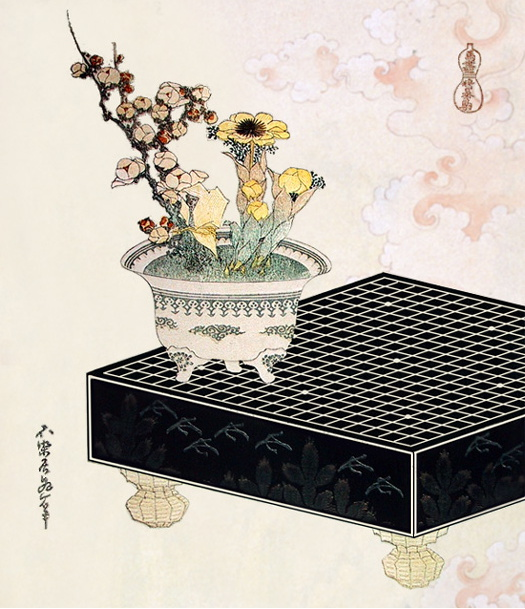
\includegraphics[width=4in]{lacquer_go_board.jpg}}
% \captionartist{Lacquer Go Board}[From the series \textit{Uma Zukushi}.]{Katsushika}{Hokusai}
% \end{figure}
%
%
%
%
% ^^A At end:
%
% \clearpage
% ^^A \pagestyle{plain}
% \phantomsection
% \tocdata{toc}{Automated}
% \addcontentsline{toc}{section}{Change History and \indexname}
%
% \pagestyle{plain}
%
% \Finale
\endinput
